%-----------------------------------------------------------------------------%
\section{Experiment and Evaluation}
\label{bab:4}
%-----------------------------------------------------------------------------%

This section evaluates \textit{ResourceDefragmentation} against the upstream \textit{HighNodeUtilization} strategy across five node-reclamation and fragmentation scenarios, using request-space Node state throughout so that placement feasibility and CPU-memory shape, rather than runtime telemetry, drive every comparison.

\subsection{Experimental Setup}
\label{sec:defrag_experimental_setup}

The experiment uses one control-plane Node and six worker Nodes. Each worker provides \(2000\,m\) allocatable CPU and approximately \(811\,Mi\) allocatable memory. Pause containers reserve declared requests while contributing negligible runtime load, allowing the experiment to control the request-space layout precisely.

The scheduler uses \textit{MostAllocated} and \textit{BalancedAllocation}. Both policies operate on identical initial workloads and namespace scope. System workloads are excluded from eviction. The drain threshold is \(0.40\), the target-utilization ceiling is \(0.90\), each scenario permits at most five Descheduler passes, and every policy-scenario cell is repeated with three seeds.

The two systems under comparison are:

\begin{itemize}
    \item \textbf{HighNodeUtilization (HNU):} the upstream utilization-based baseline with CPU and memory thresholds of \(40\%\).
    \item \textbf{ResourceDefragmentation (RD):} the proposed resource-only policy using request-based Node state, RII/FSI-based source ordering, \textit{predictSchedulerTarget}, and projected target bin score as its eviction-candidate criterion.
\end{itemize}

\subsection{Scenarios}
\label{sec:defrag_scenarios}

\begin{table*}[tbp]
    \centering
    \caption{ResourceDefragmentation Evaluation Scenarios}
    \label{tab:defrag_scenarios}
    \small
    \renewcommand{\arraystretch}{1.2}
    \begin{tabular}{l p{3.6cm} p{7.4cm}}
        \hline
        \textbf{Scenario} & \textbf{Intent} & \textbf{Initial condition} \\
        \hline
        S1 & Pure node reclamation & Uniformly underutilized Nodes whose workloads can be packed onto fewer workers. \\
        S2 & Reducible stranding & Complementary CPU-heavy and memory-heavy Nodes with no clearly high-utilization target. \\
        S3 & Mixed objective & Underutilized drain Nodes coexist with already dense balanced Nodes. \\
        S4 & Hogs and jumbo Pod & Skewed resource hogs must be merged around a large workload. \\
        S5 & Heterogeneous drain & A drain Node contains differently shaped Pods that should land on complementary targets. \\
        \hline
    \end{tabular}
\end{table*}

S1 primarily tests Node reclamation. S2 and S4 test whether dimensional fragmentation can be reduced when a scalar utilization baseline has no suitable action. S3 combines node reclamation and shape preservation. S5 isolates shape-aware eviction-candidate selection during a heterogeneous drain.

\subsection{Evaluation Metrics}
\label{sec:defrag_metrics}

The success of each policy-scenario cell is assessed through five complementary metrics that jointly capture node reclamation, dimensional balance, residual schedulability, and operational cost. Every metric operates on request-space Node state, so the cluster layout is described entirely by per-Node resource requests rather than runtime telemetry. The fundamental quantity shared by all metrics is the per-dimension utilization fraction of a worker Node \(n\):

\[
u_{n,R}
=
\frac{R_{\text{req}}(n)}
{R_{\text{alloc}}(n)},
\qquad
R \in \{\text{cpu}, \text{mem}\}
\]

Where:

\begin{itemize}
    \item \(u_{n,R}\) is the request-based utilization fraction of Node \(n\) along dimension \(R\), bounded in \([0,1]\).

    \item \(R_{\text{req}}(n)\) is the sum of resource \(R\) requested by all evictable experiment Pods assigned to Node \(n\).

    \item \(R_{\text{alloc}}(n)\) is the allocatable capacity of Node \(n\) for resource \(R\) (\(2000\,m\) CPU and approximately \(811\,Mi\) memory per worker).
\end{itemize}

%-----------------------------------------------------------------------------%
\paragraph{Active Node Count}
\label{subsubsec:defrag_metric_active}
%-----------------------------------------------------------------------------%
The Active Node Count (\(N_{\text{active}}\)) is the primary indicator of node reclamation. A worker Node is counted as active only when it hosts at least one evictable experiment workload; infrastructure namespaces such as \textit{kube-system} are excluded and therefore never keep a Node active.

\[
N_{\text{active}}
=
\sum_{n=1}^{N} a_n
\]

\[
a_n =
\begin{cases}
1, & \text{if } \sum R_{\text{req}}(n) > 0 \\
0, & \text{otherwise}
\end{cases}
\]

Where:

\begin{itemize}
    \item \(N_{\text{active}}\) is the number of worker Nodes hosting evictable experiment workloads.

    \item \(a_n\) is the binary activity indicator for Node \(n\).

    \item \(N\) is the total number of worker Nodes available in the scenario.
\end{itemize}

A reduction in \(N_{\text{active}}\) between the before- and after-snapshots indicates that one or more Nodes have been fully drained and become reclaimable for scale-down. This metric directly measures the consolidation objective and is reported as the before-and-after pair together with the number of Nodes reclaimed.

%-----------------------------------------------------------------------------%
\paragraph{Resource Stranding Score}
\label{subsubsec:defrag_metric_stranding}
%-----------------------------------------------------------------------------%
Because defragmentation optimizes the geometric \emph{shape} of utilization rather than its absolute spread, the cluster is evaluated through a stranding score that measures how far each Node deviates from per-dimension balance. The cluster stranding score \(S\) aggregates the absolute CPU-to-memory imbalance across all active Nodes:

\[
    S = \sum_{n \in N_{\text{active}}} \left|u_{n,\text{cpu}} - u_{n,\text{mem}}\right|.
\]

Where:

\begin{itemize}
    \item \(S\) is the cluster-wide resource stranding score.

    \item \(u_{n,\text{cpu}}\) and \(u_{n,\text{mem}}\) are the request-based CPU and memory utilization fractions of Node \(n\).
\end{itemize}

A Node with a large gap between its CPU and memory fractions strands the under-used dimension, since the remaining capacity cannot be allocated to a balanced reference workload. A lower \(S\) therefore indicates that CPU and memory fractions are more tightly aligned across the cluster, unlocking trapped capacity. Unlike a global standard deviation, \(S\) is insensitive to intentional differences in absolute load between Nodes and reacts only to per-Node dimensional skew.

%-----------------------------------------------------------------------------%
\paragraph{Average Active-Node Utilization}
\label{subsubsec:defrag_metric_density}
%-----------------------------------------------------------------------------%
To quantify packing density, the Average Active-Node Utilization (\(\bar{U}\)) reports the mean request-based load of the Nodes that remain active after descheduling, averaged over both resource dimensions:

\[
\bar{U}
=
\frac{1}{N_{\text{active}}}
\sum_{n : a_n = 1}
\frac{u_{n,\text{cpu}} + u_{n,\text{mem}}}{2}
\times 100\%
\]

Where:

\begin{itemize}
    \item \(\bar{U}\) is the average utilization of the surviving active Nodes, expressed as a percentage.

    \item \(N_{\text{active}}\) is the number of active Nodes after descheduling.

    \item \(\frac{u_{n,\text{cpu}} + u_{n,\text{mem}}}{2}\) is the mean per-dimension utilization fraction of Node \(n\).
\end{itemize}

A higher \(\bar{U}\) indicates that the surviving Nodes carry denser workloads, which is the expected consequence of successful consolidation. This metric complements \(N_{\text{active}}\): reclaiming Nodes is only beneficial when the retained Nodes absorb the displaced load rather than leaving the cluster uniformly sparse.

%-----------------------------------------------------------------------------%
\paragraph{Balanced Headroom}
\label{subsubsec:defrag_metric_headroom}
%-----------------------------------------------------------------------------%
The Balanced Headroom (\(H_{balanced}\)) converts residual request space into a schedulability-oriented quantity. It counts how many reference Pods, each requesting \(200\,m\) CPU and \(80\,Mi\) memory, can still be placed across the cluster after descheduling. Let \(A_{\text{cpu}}(n)\) and \(A_{\text{mem}}(n)\) denote the remaining requested CPU and memory space on Node \(n\):

\[
\begin{aligned}
H_{balanced}
&=
\sum_{n=1}^{N}
\min\!\Biggl(
\left\lfloor
\frac{A_{\text{cpu}}(n)}{c_{\text{ref}}}
\right\rfloor,\\
&\qquad\qquad
\left\lfloor
\frac{A_{\text{mem}}(n)}{m_{\text{ref}}}
\right\rfloor
\Biggr)
\end{aligned}
\]

Where:

\begin{itemize}
    \item \(H_{balanced}\) is the total number of \(200\,m/80\,Mi\) reference Pods that fit in the remaining request space.

    \item \(c_{\text{ref}} = 200\,m\) and \(m_{\text{ref}} = 80\,Mi\) are the CPU and memory requests of the balanced reference Pod.

    \item the per-Node \(\min(\cdot)\) enforces that a reference Pod fits only when both dimensions admit it, penalizing Nodes whose free capacity is stranded on a single axis.
\end{itemize}

A higher \(H_{balanced}\) indicates that defragmentation has reassembled fragmented free capacity into contiguous, jointly schedulable space. Because the per-Node term is limited by the tighter dimension, a Node with abundant free CPU but little free memory contributes little headroom, which is precisely the stranding that the policy aims to remove.

The same construction generalizes to any reference Pod shape \(r = (c_r, m_r)\), giving a family of probes \(H_r\) that reveal \emph{which} kind of capacity a layout can still admit:

\[
\begin{aligned}
H_r
&=
\sum_{n=1}^{N}
\min\!\Biggl(
\left\lfloor
\frac{A_{\text{cpu}}(n)}{c_r}
\right\rfloor,\\
&\qquad\qquad
\left\lfloor
\frac{A_{\text{mem}}(n)}{m_r}
\right\rfloor
\Biggr)
\end{aligned}
\]

In addition to the balanced probe, three skewed probes are evaluated: a CPU-skewed Pod (\(H_{cpu\text{-}skewed}\)), a memory-skewed Pod (\(H_{mem\text{-}skewed}\)), and a large jumbo Pod (\(H_{jumbo}\), \(800\,m/324\,Mi\)). The balanced probe measures general schedulability, the two skewed probes measure how much single-axis capacity remains usable, and the jumbo probe measures whether the layout retains room for large indivisible workloads. Together they show that defragmentation does not merely free aggregate space but free space of the right shape.

%-----------------------------------------------------------------------------%
\paragraph{Eviction Count and Efficiency}
\label{subsubsec:defrag_metric_eviction}
%-----------------------------------------------------------------------------%
The Eviction Count (\(E_{count}\)) measures the operational cost of a descheduling sweep as the total number of Pods relocated, extracted from the Descheduler job log:

\[
E_{count}
=
\sum_{j \in J} e_j
\]

Where:

\begin{itemize}
    \item \(E_{count}\) is the total number of Pods evicted across all passes of a sweep.

    \item \(J\) is the set of log entries recorded during the job lifecycle.

    \item \(e_j\) is a binary flag equal to \(1\) when log entry \(j\) records an eviction, and \(0\) otherwise.
\end{itemize}

Efficiency is interpreted jointly from \(E_{count}\), the number of Nodes reclaimed (\(\Delta N_{\text{active}}\)), and the reduction in stranding (\(\Delta S\)). A policy is more efficient when it achieves the same structural improvement, that is, the same reclamation and balance gain, with fewer Pod movements, since every eviction imposes disruption on the running workload.

%-----------------------------------------------------------------------------%
\paragraph{Convergence and Safety}
\label{subsubsec:defrag_metric_safety}
%-----------------------------------------------------------------------------%
Finally, each run is validated for convergence and safety. The per-pass eviction count must eventually reach zero within the bounded loop of at most five passes, confirming that the policy reaches a stable fixed point rather than oscillating. After each run, every Pod must remain schedulable, so no after-snapshot may contain a Pending Pod, and no eviction request may remain stuck beyond the evicted Pods recorded in the log. These conditions verify that the consolidation pressure is exercised without violating feasibility or workload availability.

\subsection{Node Reclamation}
\label{sec:defrag_node_reclamation}

\begin{table*}[tbp]
    \centering
    \caption{Active Worker Nodes Before and After Descheduling}
    \label{tab:defrag_node_reclamation}
    \small
    \renewcommand{\arraystretch}{1.2}
    \begin{tabular}{@{}l c c c c@{}}
        \hline
        \textbf{Scenario} & \textbf{HNU} & \textbf{Reclaimed} & \textbf{RD} & \textbf{Reclaimed} \\
        \hline
        S1 & \(6 \rightarrow 6\) & \(0\) & \(6 \rightarrow 2\) & \(\mathbf{4}\) \\
        S2 & \(6 \rightarrow 6\) & \(0\) & \(6 \rightarrow 3\) & \(\mathbf{3}\) \\
        S3 & \(6 \rightarrow 4\) & \(\mathbf{2}\) & \(6 \rightarrow 5\) & \(1\) \\
        S4 & \(5 \rightarrow 5\) & \(0\) & \(5 \rightarrow 4\) & \(\mathbf{1}\) \\
        S5 & \(4 \rightarrow 3\) & \(1\) & \(4 \rightarrow 3\) & \(1\) \\
        \hline
    \end{tabular}
\end{table*}

\begin{figure*}[tbp]
    \centering
    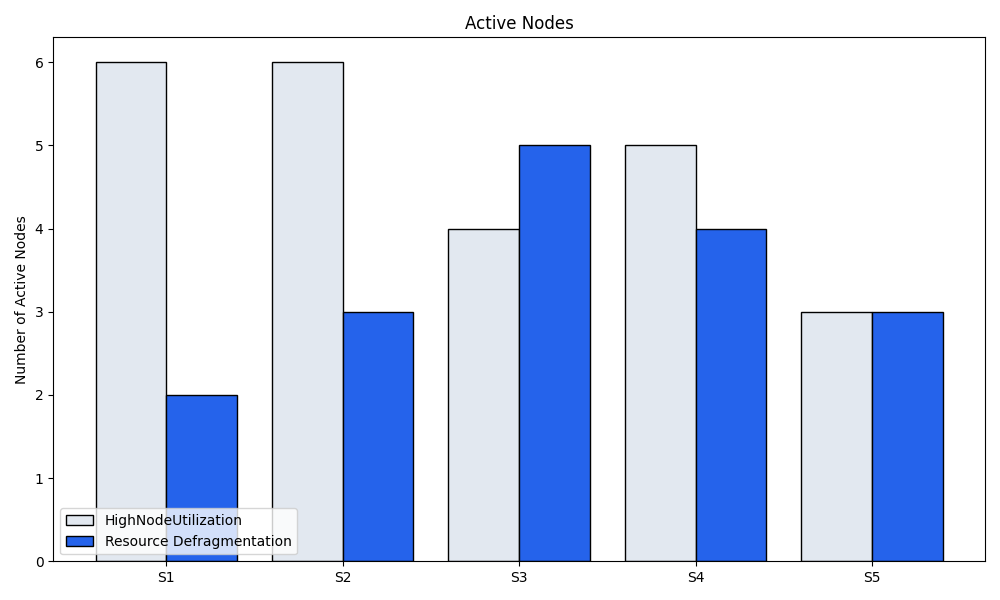
\includegraphics[width=0.95\textwidth]{assets/pics/defrag/chart_active_nodes.png}
    \caption{Active worker Nodes per scenario after descheduling.}
    \label{fig:defrag_active_nodes}
\end{figure*}

ResourceDefragmentation reclaims four Nodes in S1 and three in S2, while HNU performs no eviction in either scenario, as shown in Figure \ref{fig:defrag_active_nodes}. HNU requires Nodes above its threshold to act as packing targets; uniformly low or uniformly fragmented layouts therefore produce no action. ResourceDefragmentation instead treats sparse Nodes and low bin-quality Nodes as resource-only consolidation sources, then uses \textit{predictSchedulerTarget} to choose Pods with feasible denser targets even when the baseline cannot form high- and low-utilization groups.

S3 is the only reclamation case won by HNU. Dense balanced targets already exist, allowing the threshold policy to drain two Nodes greedily. ResourceDefragmentation respects the \(0.90\) ceiling and reclaims one Node. S5 is especially useful because both policies reclaim the same Node, allowing placement quality and eviction cost to distinguish them.

The consolidation effect is also visible in the density of the surviving Nodes. Figure \ref{fig:defrag_avg_utilization} reports the average active-Node utilization \(\bar{U}\) after descheduling: in the consolidation and fragmentation scenarios ResourceDefragmentation drives the retained Nodes to substantially higher density than HNU, confirming that the reclaimed capacity is absorbed rather than left uniformly sparse.

\begin{figure*}[tbp]
    \centering
    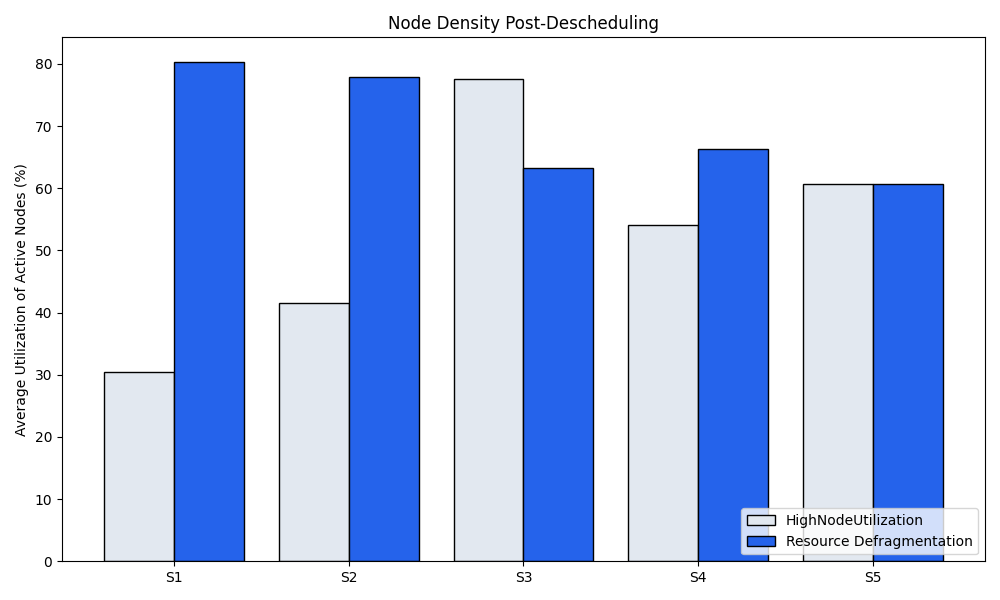
\includegraphics[width=0.95\textwidth]{assets/pics/defrag/chart_avg_utilization.png}
    \caption{Average utilization of active Nodes after descheduling (\(\bar{U}\)).}
    \label{fig:defrag_avg_utilization}
\end{figure*}

\subsection{Stranding Reduction}
\label{sec:defrag_stranding_results}

\begin{table*}[tbp]
    \centering
    \caption{Cluster Stranding Score Before and After Descheduling}
    \label{tab:defrag_stranding}
    \renewcommand{\arraystretch}{1.2}
    \begin{tabular}{@{}l c c@{}}
        \hline
        \textbf{Scenario} & \textbf{HighNodeUtilization} & \textbf{ResourceDefragmentation} \\
        \hline
        S1 & \(0.049 \rightarrow 0.049\) & \(0.049 \rightarrow 0.050\) \\
        S2 & \(3.727 \rightarrow 3.727\) & \(3.727 \rightarrow \mathbf{0.971}\) \\
        S3 & \(1.395 \rightarrow 1.408\) & \(1.395 \rightarrow \mathbf{1.386}\) \\
        S4 & \(3.243 \rightarrow 3.243\) & \(3.243 \rightarrow \mathbf{1.112}\) \\
        S5 & \(1.338 \rightarrow 1.298\) & \(1.338 \rightarrow \mathbf{0.123}\) \\
        \hline
    \end{tabular}
\end{table*}

\begin{figure*}[tbp]
    \centering
    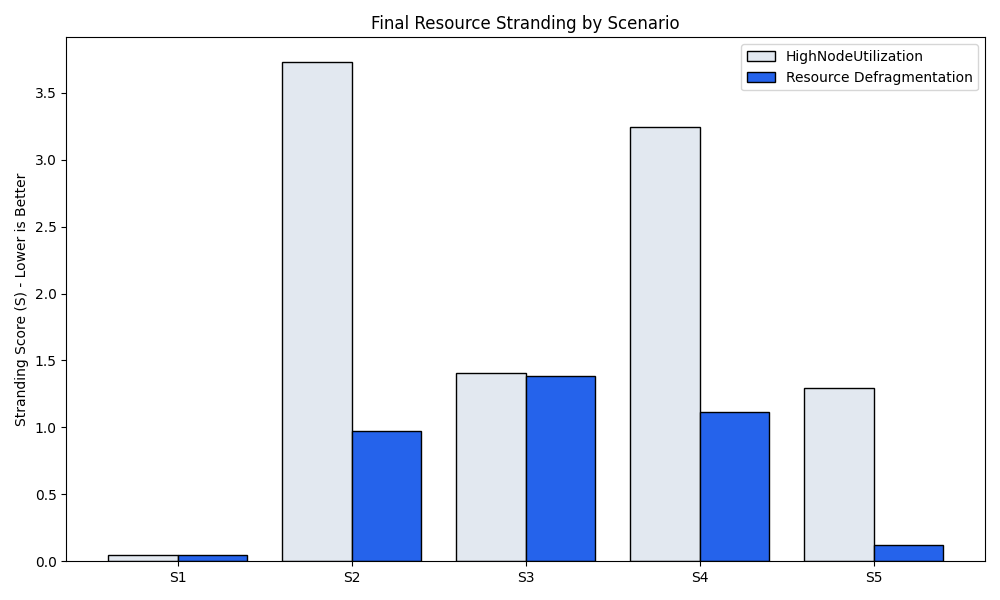
\includegraphics[width=0.95\textwidth]{assets/pics/defrag/chart_stranding.png}
    \caption{Final cluster stranding score \(S\) per scenario (lower is better).}
    \label{fig:defrag_stranding}
\end{figure*}

As summarized in Figure \ref{fig:defrag_stranding}, the result separates node reclamation from dimensional defragmentation. S1 begins with little stranding, so packing four Nodes into two leaves \(S\) essentially unchanged. In S2 and S4, ResourceDefragmentation uses the predicted-target score to combine complementary shapes and reduces \(S\) by approximately \(74\%\) and \(66\%\), respectively; HNU does not act.

In S3, HNU reclaims one additional Node but slightly worsens \(S\), whereas ResourceDefragmentation reduces it from \(1.395\) to \(1.386\). This shows the consequence of retaining resource shape in the target objective rather than optimizing Node count alone.

\subsection{S5 Heterogeneous-Drain Analysis}
\label{sec:defrag_s5_analysis}

S5 tests whether the selector distinguishes Pods on the same source Node by the shape of their predicted destinations. The source contains CPU-heavy and memory-heavy candidates, while other active Nodes expose complementary residual capacity.

ResourceDefragmentation predicts a feasible target for each candidate and compares projected target bin scores after applying the ceiling and pack-upward guards. It moves the CPU-shaped Pod to the Node with spare CPU-compatible balance and the memory-shaped Pod to the complementary Node. The source becomes empty after two evictions, and the receiving Nodes end in nearly balanced states. Consequently, \(S\) falls from \(1.338\) to \(0.123\), a reduction of approximately \(91\%\).

HNU also empties one Node, but it requires three evictions and only reduces \(S\) to \(1.298\). Thus, equal Node reclamation does not imply equal defragmentation quality. The predicted-target criterion produces both a better placement and lower disruption.

\subsection{Headroom and Eviction Efficiency}
\label{sec:defrag_headroom_efficiency}

\begin{table*}[tbp]
    \centering
    \caption{Balanced Headroom and Eviction Count}
    \label{tab:defrag_headroom_efficiency}
    \renewcommand{\arraystretch}{1.2}
    \begin{tabular}{@{}l c c c c@{}}
        \hline
        \textbf{Scenario} & \textbf{HNU \(H_{balanced}\)} & \textbf{HNU Evict.} & \textbf{RD \(H_{balanced}\)} & \textbf{RD Evict.} \\
        \hline
        S1 & \(42\) & \(0\) & \(39\) & \(10\) \\
        S2 & \(15\) & \(0\) & \(\mathbf{29}\) & \(6\) \\
        S3 & \(18\) & \(4\) & \(\mathbf{19}\) & \(2\) \\
        S4 & \(13\) & \(0\) & \(\mathbf{24}\) & \(5\) \\
        S5 & \(32\) & \(3\) & \(\mathbf{38}\) & \(\mathbf{2}\) \\
        \hline
    \end{tabular}
\end{table*}

\begin{figure*}[tbp]
    \centering
    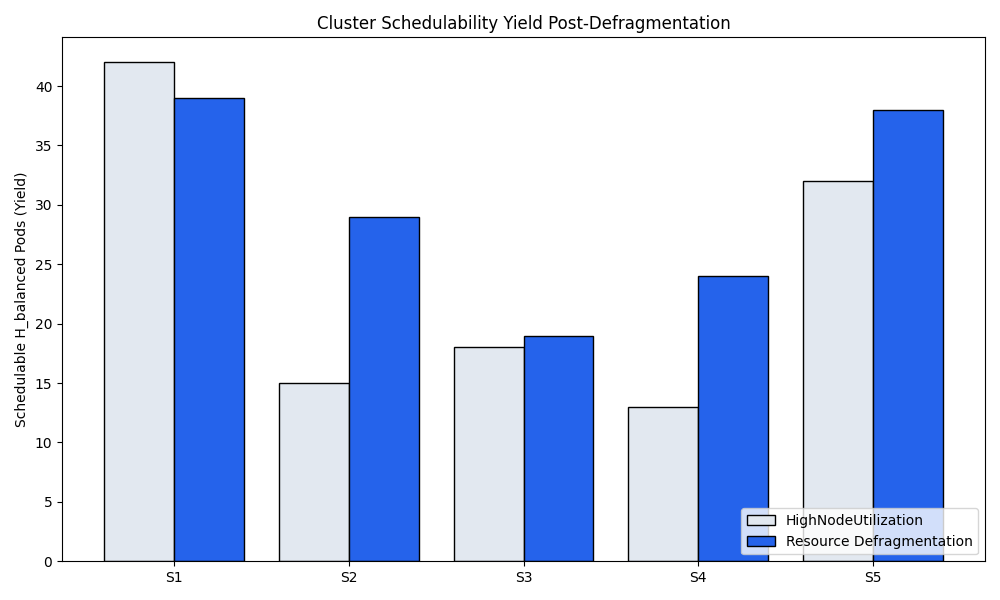
\includegraphics[width=0.95\textwidth]{assets/pics/defrag/chart_h_balanced.png}
    \caption{Balanced headroom \(H_{balanced}\) per scenario after descheduling.}
    \label{fig:defrag_h_balanced}
\end{figure*}

HNU retains higher distributed headroom in S1 because it leaves all six Nodes active; this is not a node reclamation success. In the fragmentation scenarios, ResourceDefragmentation exposes substantially more balanced headroom, as shown in Figure \ref{fig:defrag_h_balanced}. S5 is the strongest efficiency result: two ResourceDefragmentation evictions reclaim one Node, reduce \(S\) by \(1.215\), and leave headroom for 38 balanced reference Pods. HNU uses three evictions for the same reclamation, reduces \(S\) by only \(0.040\), and leaves headroom for 32 reference Pods.

The eviction cost behind these gains is reported in Figure \ref{fig:defrag_evictions}. ResourceDefragmentation spends evictions only where consolidation or defragmentation is achievable, and in S3 and S5 it reaches an equal or better cluster state than HNU with fewer Pod movements.

\begin{figure*}[tbp]
    \centering
    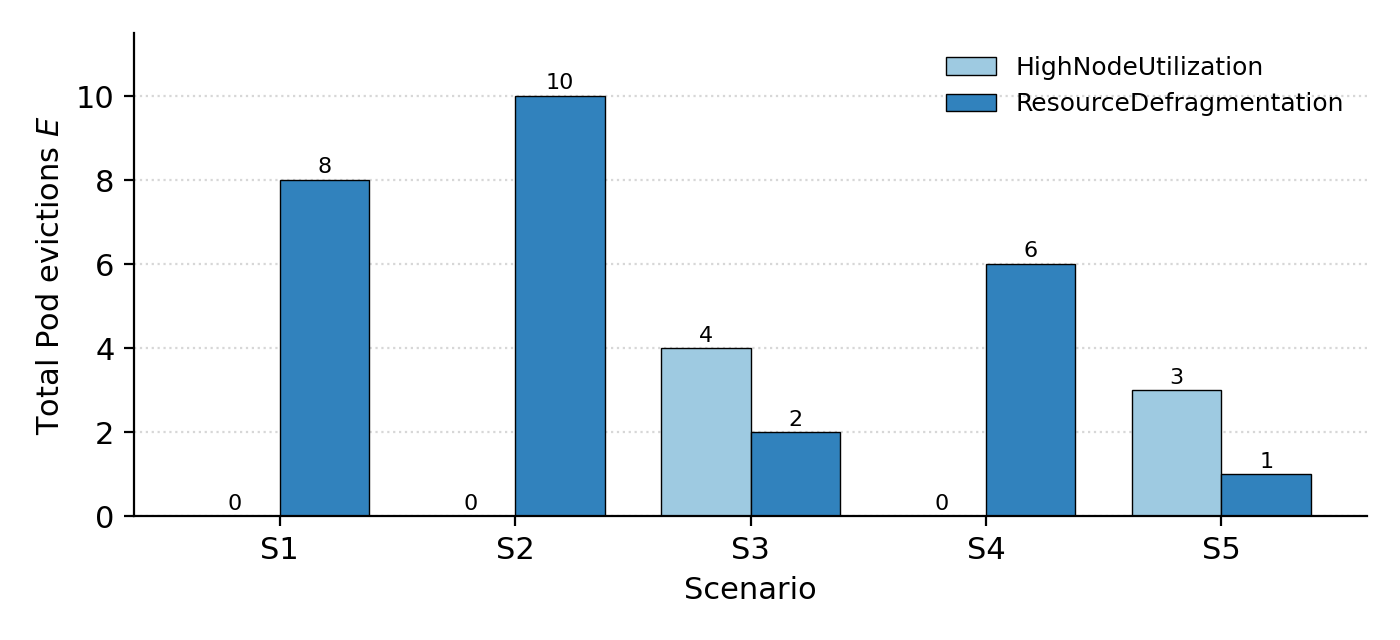
\includegraphics[width=0.95\textwidth]{assets/pics/defrag/chart_evictions.png}
    \caption{Total Pod evictions per scenario (\(E_{count}\)).}
    \label{fig:defrag_evictions}
\end{figure*}

\subsection{Shape-Specific Schedulability Yield}
\label{sec:defrag_shape_headroom}

Balanced headroom alone does not show \emph{which} kind of workload a defragmented layout can still admit. To make this explicit, the residual capacity is also probed with three skewed reference Pods: a CPU-skewed Pod, a memory-skewed Pod, and a large jumbo Pod (\(800\,m/324\,Mi\)). Table \ref{tab:defrag_shape_headroom} reports the resulting yields after descheduling.

\begin{table*}[tbp]
    \centering
    \caption{Schedulability Yield by Reference-Pod Shape After Descheduling}
    \label{tab:defrag_shape_headroom}
    \small
    \renewcommand{\arraystretch}{1.2}
    \begin{tabular}{l cc cc cc}
        \hline
        & \multicolumn{2}{c}{\textbf{CPU-skewed}} & \multicolumn{2}{c}{\textbf{Memory-skewed}} & \multicolumn{2}{c}{\textbf{Jumbo}} \\
        \textbf{Scenario} & \textbf{HNU} & \textbf{RD} & \textbf{HNU} & \textbf{RD} & \textbf{HNU} & \textbf{RD} \\
        \hline
        S1 & \(12\) & \(\mathbf{13}\) & \(12\) & \(\mathbf{13}\) & \(6\) & \(\mathbf{8}\) \\
        S2 & \(9\)  & \(9\)          & \(9\)  & \(\mathbf{11}\) & \(0\) & \(\mathbf{6}\) \\
        S3 & \(\mathbf{6}\) & \(5\)   & \(6\)  & \(\mathbf{9}\)  & \(\mathbf{4}\) & \(2\) \\
        S4 & \(4\)  & \(\mathbf{8}\)  & \(4\)  & \(\mathbf{7}\)  & \(3\) & \(\mathbf{4}\) \\
        S5 & \(\mathbf{12}\) & \(11\) & \(11\) & \(11\)          & \(6\) & \(\mathbf{7}\) \\
        \hline
    \end{tabular}
\end{table*}

In the fragmentation scenarios, ResourceDefragmentation increases the yield for skewed and jumbo workloads where it matters most. In S2 and S4, where complementary CPU-heavy and memory-heavy Nodes are merged, it lifts memory-skewed yield (\(9 \to 11\) in S2, \(4 \to 7\) in S4) and restores jumbo capacity that the baseline cannot provide at all in S2 (\(0 \to 6\)), as shown in Figures \ref{fig:defrag_h_cpu_skewed}, \ref{fig:defrag_h_mem_skewed}, and \ref{fig:defrag_h_jumbo}. In S5 it matches or slightly exceeds the baseline on every shape while using fewer evictions.

The two cases where HNU leads, CPU-skewed and jumbo yield in S3, reflect the same trade-off seen in the balanced headroom and stranding results: HNU empties an additional Node by greedily packing onto pre-dense targets, which leaves more whole-Pod slots free but at a slightly worse stranding score. ResourceDefragmentation instead preserves resource shape, so its remaining capacity is more evenly balanced across dimensions rather than concentrated on one emptied Node.

\begin{figure*}[tbp]
    \centering
    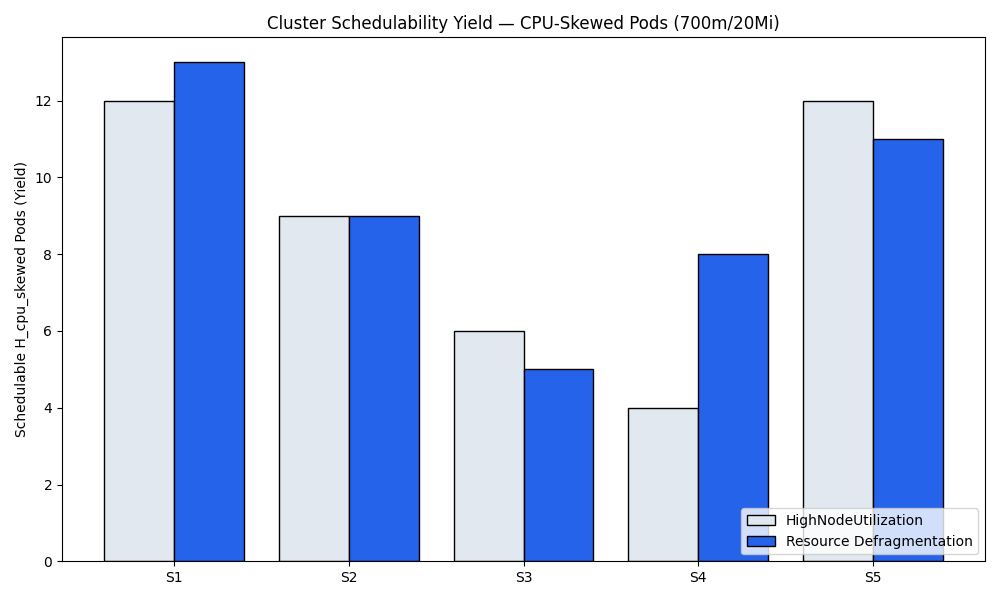
\includegraphics[width=0.95\textwidth]{assets/pics/defrag/chart_h_cpu_skewed.png}
    \caption{CPU-skewed schedulability yield \(H_{cpu\text{-}skewed}\) per scenario after descheduling.}
    \label{fig:defrag_h_cpu_skewed}
\end{figure*}

\begin{figure*}[tbp]
    \centering
    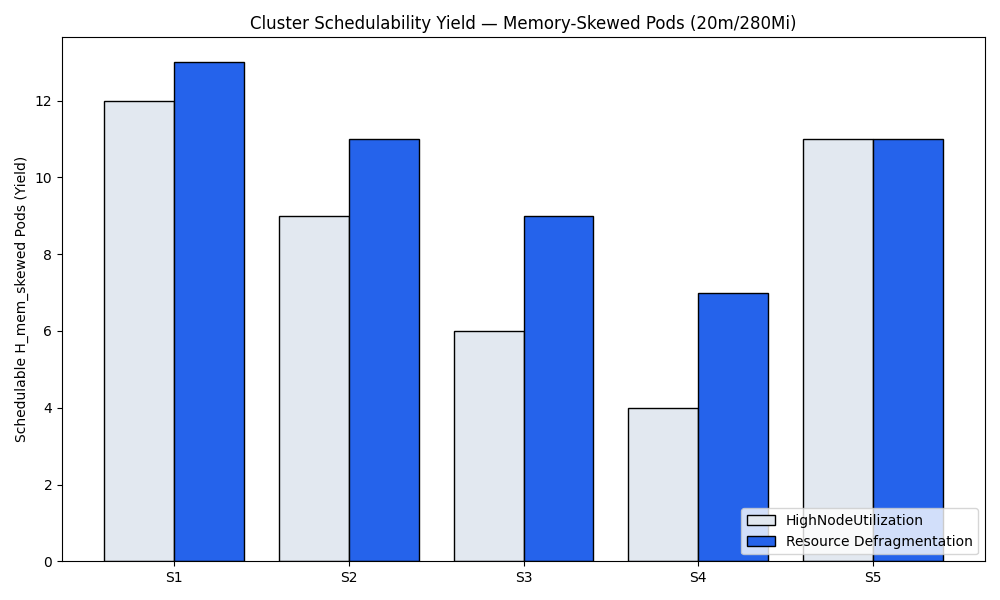
\includegraphics[width=0.95\textwidth]{assets/pics/defrag/chart_h_mem_skewed.png}
    \caption{Memory-skewed schedulability yield \(H_{mem\text{-}skewed}\) per scenario after descheduling.}
    \label{fig:defrag_h_mem_skewed}
\end{figure*}

\begin{figure*}[tbp]
    \centering
    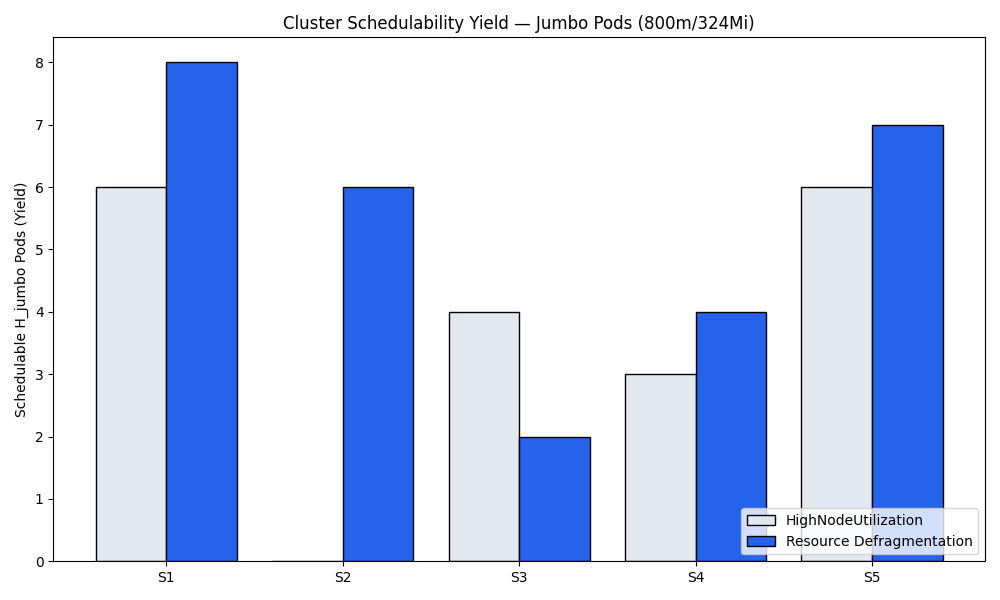
\includegraphics[width=0.95\textwidth]{assets/pics/defrag/chart_h_jumbo.png}
    \caption{Jumbo (\(800\,m/324\,Mi\)) schedulability yield \(H_{jumbo}\) per scenario after descheduling.}
    \label{fig:defrag_h_jumbo}
\end{figure*}

\subsection{Convergence and Safety}
\label{sec:defrag_convergence_safety}

\begin{table*}[tbp]
    \centering
    \caption{Representative Per-Pass Eviction Counts}
    \label{tab:defrag_convergence}
    \begin{tabular}{@{}l c c@{}}
        \hline
        \textbf{Scenario} & \textbf{HighNodeUtilization} & \textbf{ResourceDefragmentation} \\
        \hline
        S1 & \(0\) & \(8, 2, 0\) \\
        S2 & \(0\) & \(6, 0\) \\
        S3 & \(4, 0\) & \(2, 0\) \\
        S4 & \(0\) & \(4, 1, 0\) \\
        S5 & \(3, 0\) & \(2, 0\) \\
        \hline
    \end{tabular}
\end{table*}

Every scenario converges to a zero-eviction pass within two or three passes, with no oscillation. Across all repetitions, no after-snapshot contains a Pending Pod. All evicted Pods are controller-owned and eligible under the default evictor, infrastructure namespaces are excluded, and no eviction request remains outstanding. These observations validate the feasibility guard, target ceiling, and bounded execution loop.

\subsection{Resource Policy Findings}
\label{sec:defrag_findings}

The evaluation yields four main findings:

\begin{itemize}
    \item ResourceDefragmentation consolidates uniformly underutilized and uniformly fragmented layouts in which HNU is a no-op.
    \item ResourceDefragmentation reduces dimensional stranding in S2, S4, and S5 while preserving or increasing balanced schedulability headroom.
    \item Predicted-target bin-score selection is especially effective for heterogeneous drain Nodes, reducing S5 stranding from \(1.338\) to \(0.123\) with two evictions.
    \item The policy converges without leaving Pods Pending, showing that node reclamation pressure can be combined with explicit feasibility and utilization guards.
\end{itemize}
